\chapter{Variable Structure Control}
Nonlinear control strategy where
\begin{itemize}
\item a discontinuous feedback control law is designed that forces the state of the system to reach and then remain on a certain surface (the sliding surface);
\item the dynamic of the system restricted to the sliding surface is controlled so as to produce a desired behaviour, i.e., convergence to some pre-defined point.
\end{itemize}
It is also known as sliding mode control. Let's introduce the topic with an example.
\paragraph{Example [S.V. Emilianov]}
\[
s:\begin{cases}
	\dot{x}_1=_2\\
	\dot{x}_2=-x_1+2x_2+u\qquad \text{linear system}\\
	y=x_1
\end{cases}
\]
\[
C:u=-\psi(x)y\qquad \text{switching controller}
\]where $\psi(x)=\begin{cases}
	-4,\quad s(x<0)\\
	+4,\quad s(x)>0
\end{cases},\qquad s(x)=x_1(0.5x_1+x_2)$.
System $\Sigma$ has a variable structure
\begin{figure}[H]
	\centering
	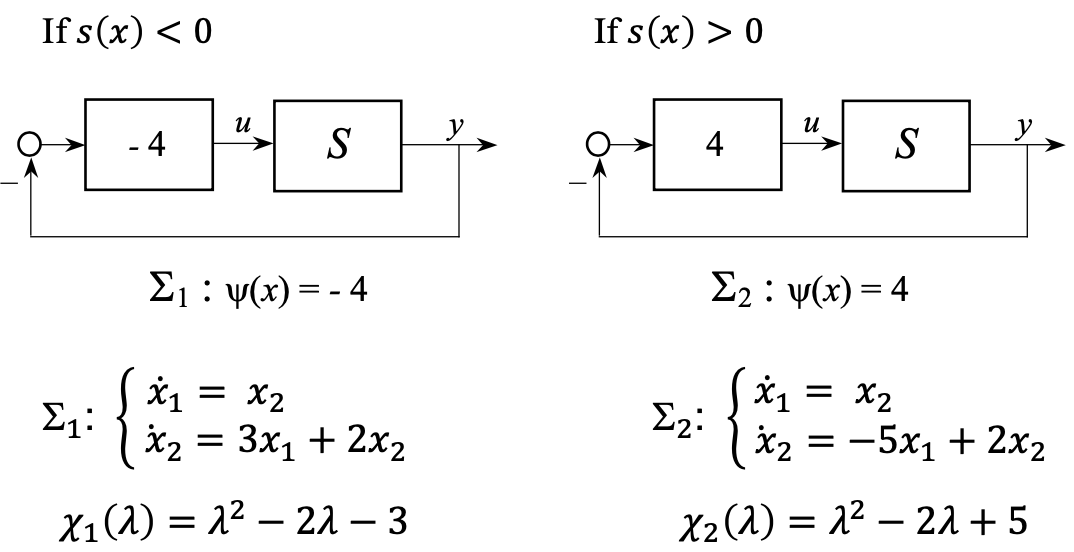
\includegraphics[scale=0.4]{immagini/es6}
	\caption{}
	\label{fig:es6}
\end{figure}
Since the switching signal is of the second order we have two switching surfaces:
\[
s(x):=x_1(0.5x_1+x_2) \Leftrightarrow \begin{cases}
	x_1=0\\0.5x_1+x_2=0
\end{cases}
\]

\begin{figure}[H]
	\centering
	\begin{subfigure}[b]{0.3\textwidth}
		\centering
		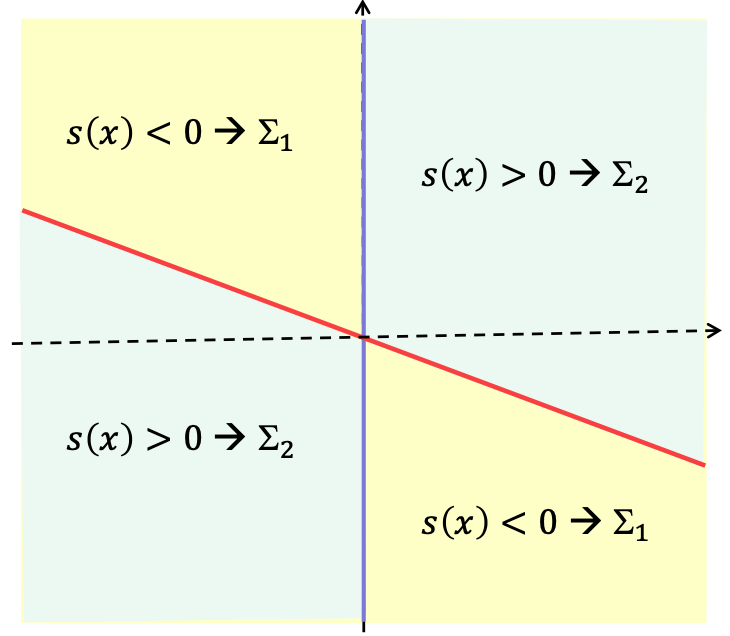
\includegraphics[scale=0.25]{immagini/es61}
		\caption{Switching surfaces}
		\label{fig:es61}
	\end{subfigure}
	\hfill
	\begin{subfigure}[b]{0.3\textwidth}
		\centering
		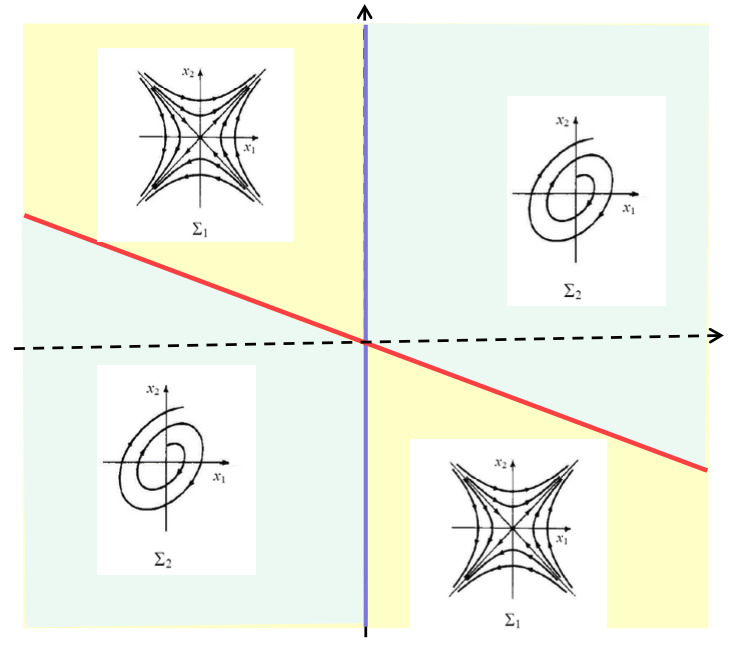
\includegraphics[scale=0.25]{immagini/es62}
		\caption{Different trajectories}
		\label{fig:es62}
	\end{subfigure}
	\hfill
	\label{fig:asdf}
\end{figure}
Combining the trajectories we end up in the following situation
\begin{figure}[H]
	\centering
	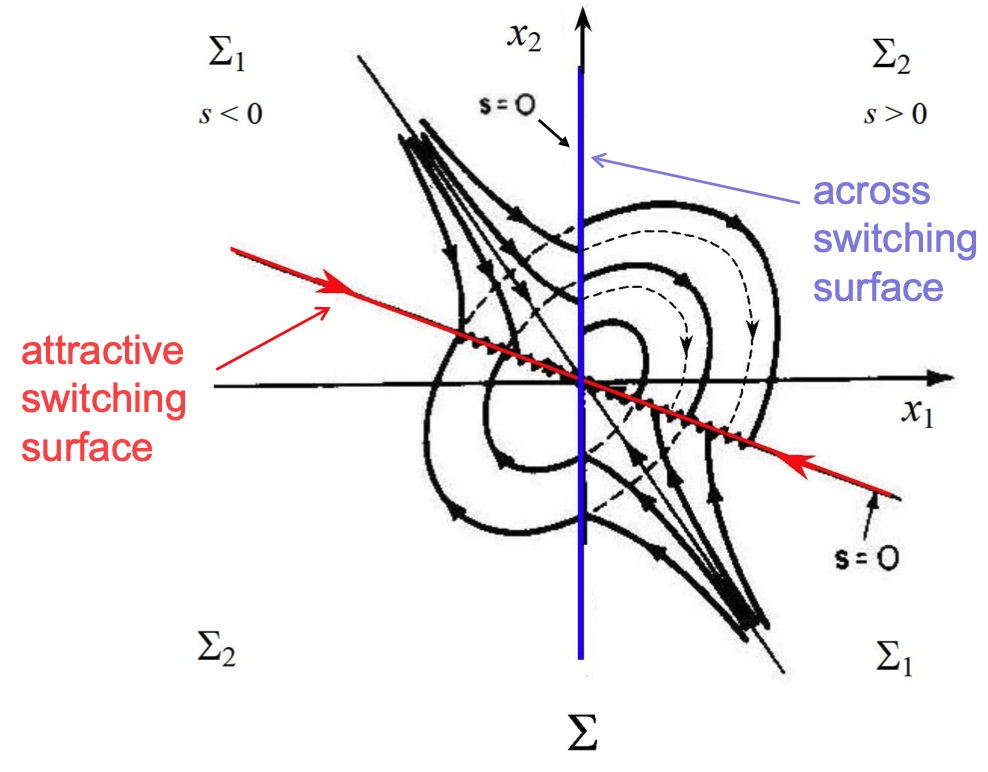
\includegraphics[scale=0.4]{immagini/es63}
	\caption{}
	\label{fig:es63}
\end{figure}
In each quadrant is represented its correspondent the dynamic. In $x_1=0$ we have a continuation of the dynamic between the two sector so we are encountering an \emph{across} switching surface. While, when we encouter the other switching surface the two trajectories are approaching one another so we can't actually leave the switching surface. In this case we have approached an \emph{attractive} switching function.
As we saw in this example, conceptually there are two type of switching surfaces:
\begin{itemize}
	\item \textcolor{blue}{Across switching surface}: the state reaches the surface S while following some dynamics, crosses it, and continues its evolution according to the other dynamics.
	\begin{figure}[H]
		\centering
		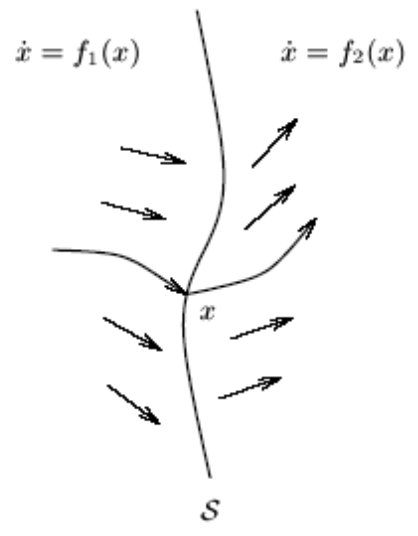
\includegraphics[scale=0.4]{immagini/es4}
		\caption{Across switching surface}
		\label{fig:es4}
	\end{figure}
	\item \textcolor{red}{Attractive switching surface}: the state reaches the surface S and cannot leave it because the vector fields on both sides are pointing towards S
	$\to$ It can only slide along S (sliding mode)
	\begin{figure}[H]
		\centering
		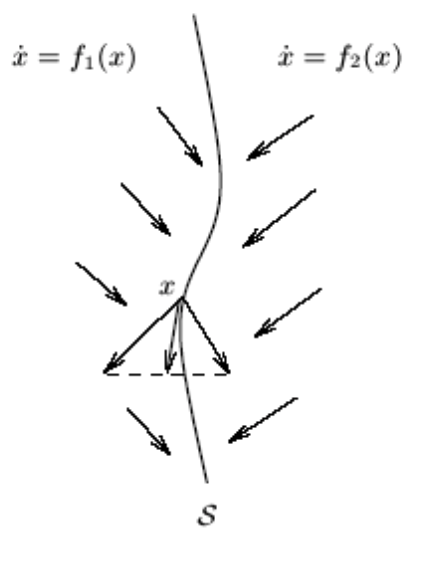
\includegraphics[scale=0.4]{immagini/es65}
		\caption{Attractive switching surface}
		\label{fig:es65}
	\end{figure}
\end{itemize}
 reaching the surface $0.5 x_1+x_2=0$ the state is constrained to evolve on that surface. In practice this mean that we are passing from a second order system to a one degree one (we are moving on a line).
 \[
 \begin{cases}
 	\dot{x_1}=x_2\\
 	\dot{x}_2=-x_1+2x_2+u\qquad x_2=-0.5x_1\\
 	y=x1
 \end{cases}
 \]
 \[\Downarrow\]\[\dot{x}_1=-0.5x_1\] 
 
This dynamic is asymptotically stable since $x_1$ tends to zero.
\section{The basics}
Given a linear-time-invariant SISO system of order n $S:\begin{cases}
	\dot{x}=Ax+Bu\\y=Cx
\end{cases}$ with (A,B) controllable and (A,C) observable, design a variable structure controller such that y(t) tends to some constant reference signal y°, for all y° and for all x(0). \\ A fundamental condition is to have the system S in the \emph{controllable canonical form} and if it is not given in this form we have to reconduct ourselves to that. Look Section \ref{canonical} for the controllable canonical form structure.
\paragraph{Design procedure} We can concretely identify two main steps for this technique:	
\begin{enumerate}
	\item determine a switching function 
	\[
	s(\cdot):\Re^n\to\Re
	\]
	such that S constrained on the sliding surface s(x)=0 converges to a (pseudo-)equilibrium with y=y°;
	\item Determine a control law u=k(x;y°) such that all the state trajectories starting from outside the sliding surface cross that surface in finite time [reaching condition].
\end{enumerate}
\section{Choice of the switching function}
Typical choice (not only for linear system) for the switching function: 
\[
s(x):=\beta_{n-1}x_1+\beta_{n-2}x_2+\dots+\beta_1x_{n-1}+x_n-\bar{w}
\]
 Then, the system dynamics on the sliding surface s(x)=0 is given by 
\[
\begin{cases}
	\dot{x}_i=x_{i+1},\qquad i=1,2,\dots,n-2\\
	\dot{x}_{n-1}=x_n=-\beta_{n-1}x_1-\beta_{n-2}x_2-\dots-\beta_1x_{n-1}+x_n+\bar{w}
\end{cases}
\]So the resulting system has n-1 dimension. $\bar{w}$ is our degree of freedom used to impose y=y°. The characteristic polynomial is 
\[
\chi^*(\lambda)=\lambda^{n-1}+\beta_1\lambda^{n-2}+\dots+\beta_{n-1}
\]
When we are in the switching surface we can impose the dynamics of the system by arbitrarily choosing the value of the coefficients of $\chi^*$ in order to have the roots matching with the one of the desired one. If all the roots have \underline{strictly negative} real part (thus, $\beta_{n-1}\neq0$), then, S* is asymptotically stable and admits a single equilibrium for each value for $\bar{w}$.
\begin{note}
	If $\beta_{n-1}=0$ one root is s=0. Moreover $b_n$ has to be different from 0 to have a well defined control problem.
\end{note}
Let's analyze the equilibrium setting the righten side of the equations equal to zero.
\[
\bar{x}_1=\frac{\bar{w}}{\beta_{n-1}}\qquad \bar{x}_i=0,\quad i=2,3,\dots,n-1
\] is the only asymptotically stable equilibrium of \[
S^*:\quad \begin{cases}
	\dot{x}_i=x_{i+1},\qquad i=1,2,\dots,n-2\\
	\dot{x}_{n-1}=x_n=-\beta_{n-1}x_1-\beta_{n-2}x_2-\dots-\beta_1x_{n-1}+\bar{w}
\end{cases}
\]Correspondingly $\bar{x}_n=0$ because the system dimension is $n-1$,
\[
	\bar{y}=C\bar{x}=b_n\bar{x}_1=\bar{w}\frac{b_n}{\beta_{n-1}}.
\]If we set $\bar{w}=\gamma y°$, $\gamma:=\frac{\beta_{n-1}}{b_n}$ then $\bar{y}=y°$.
So, since now we have done the first part defining a switching function s(x)  such that when the system evolves along s(x)=0 it reaches in finite time the eigenvalues we have imposed through s(x). Let's skip now to the second part.
\section{Reaching condition}
First of all specify the dynamics of the switching function $s(x(t))$ so that the Lyapunov-like function $V(s)=\frac{1}{2}s^2$, has negative time derivative satisfying \[\frac{dV}{dt}=s\dot{s}\le -\eta |s|,\qquad \eta>0\] then we are going to get that s becomes 0 in fintie time independently of s(0).\\
\underline{Statement:}\\ If such condition on V(s) holds, then, for any initial condition $x(0)$, $s(x(t))$ converges to zero in finite time.
\begin{proof}
	Given that $V(s)=\frac{1}{2}s^2$, \[\frac{dV}{dt}=s\dot{s}\le -\eta |s|=-\eta\sqrt{2V}\]The die is that if we divide the left-hand side by $2\sqrt{V}$ it will be easy to integrate and solve the equation.\[
	\int_{0}^{t}\frac{1}{2}\frac{\dot{V}}{\sqrt{V}}dt\ge\int_{0}^{t}- \frac{\eta}{\sqrt{2}}dt\to\sqrt{V(t)}-\sqrt{V(0)}\le-\frac{\eta}{\sqrt{2}}t
\] This can be rewritten as \[
\frac{1}{\sqrt{2}}|s(x(t))|\le -\frac{\eta}{\sqrt{2}}t+\frac{1}{\sqrt{2}}|s(x(0))|
\]So the time t required for the switching function to go to zero if the condition above is satisfied is upper bounded by \[t_r\le\frac{|s(x(0))|}{\eta}\]
\end{proof}
Now comes the  interesting part: how do we choose the dynamics of s such that the condition of before is satisfied?
Dynamics of the switching function:
\[\dot{s}=-q \, sgn(s)-r \, g(s)\] with $q>0$ and $r\ge0$, and $g(\cdot)$ such that $sg(s)>0,\forall s\neq 0$.\begin{figure}[H]
	\centering
	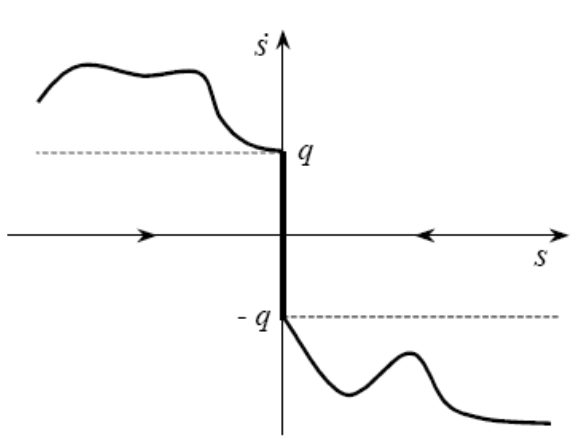
\includegraphics[scale=0.4]{immagini/vscgraph}
	\caption{$\begin{cases}-r \, g(s)>0,\qquad s<0\\-r \, g(s)<0,\qquad s>0\end{cases}$}
	\label{fig:vscgraph}
\end{figure}
$\dot{s}>q>0$ when $s<0$ and $\dot{s}<-q<0$ when $s>0$. s=0 is reached in finite time.\\The condition for finite time convergence to the switching surface is satisfied with $\eta=q$:\[
\frac{dV}{dt}=s\dot{s}=-q \, sgn(s)s-r \, s	\, g(s)=-q|s|-r	\, s \, g(s)\le-q|s|
\]The time to convergence satisfies \[t_r\le\frac{|s(x(0))|}{q}\]What is the control law that imposes this dynamics to s(t)?\\
Recalling the definition of the switching function s(x):\[s(x):=\beta_{n-1}x_1+\beta_{n-2}x_2+\dots+\beta_1x_{n-1}+x_n-\bar{w}\] which can be rewritten in compact form as:
\[s(x)=\beta'x-\gamma y°,\qquad \beta':=\begin{bmatrix}
	\beta_{n-1} & \beta_{n-2} & \dots & \beta_1 & 1
\end{bmatrix}, \quad \dot{s}=\beta'\dot{x}=\beta'(Ax+Bu).\] Follows that \[
\beta'(Ax+Bu)=-qsgn(s(x))-rg(s(x))
\] since in controllable canonical form matrix B is: 
\[B=\begin{bmatrix}
	0 \\ 0 \\ 0 \\ \vdots \\0 \\ 1
\end{bmatrix}
\] and so $\beta'B=1$ then follows that
\[\begin{aligned}
	u&=-(\beta'Ax+q sgn(\beta'x-\gamma y°)+rg(\beta'x-\gamma y°))\\
	&=-\alpha'x+q sgn(\gamma y°-\beta'x)+rg(\gamma y°-\beta'x)
\end{aligned}
\] where $-g(s)=g(-s) $ is an odd function and $\alpha'=\beta'A$. We can rewrite the equation in the following way:\[
u=-\alpha'x+qsgn(-s)+rg(-s)
\] where $s=\beta'x-\gamma y°$.
\begin{figure}[H]
	\centering
	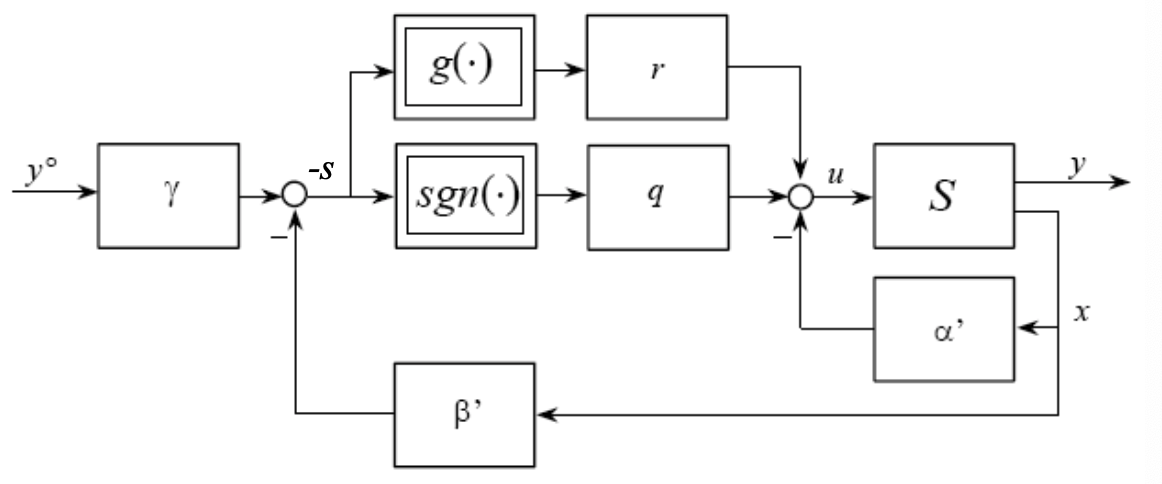
\includegraphics[scale=0.4]{immagini/nonso}
	\caption{}
	\label{fig:nonso}
\end{figure}
\begin{note}
	In order to avoid infinitely fast switching the ''sgn'' function is implemented as a 2-level hysteresis switching controller with M=1 and B tends to 0.
	\begin{figure}[H]
		\centering
		\begin{subfigure}[b]{0.3\textwidth}
			\centering
			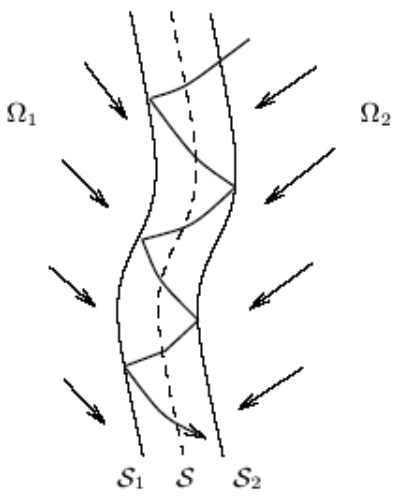
\includegraphics[scale=0.25]{immagini/nota61}
			\caption{Switching dynamics}
			\label{fig:nota61}
		\end{subfigure}
		\hfill
		\begin{subfigure}[b]{0.3\textwidth}
			\centering
			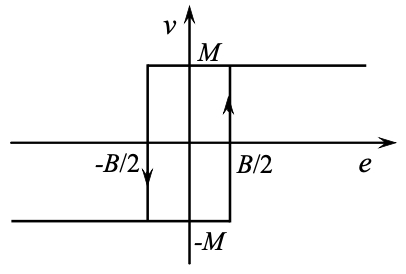
\includegraphics[scale=0.25]{immagini/nota62}
			\caption{Hysteresis function}
			\label{fig:hyste}
		\end{subfigure}
		\hfill
		\label{fig:notachap6}
		\caption[]{}
	\end{figure}
\end{note}
\section{A numerical example}
Let's introduce now a numerical example.\[G(s)=\frac{-400(s+5)}{(s^2+5s+20)(s+10)(s-1)}=\frac{-400(s+5)}{s^4+14s^3+55s^2+130s-200}\]
\begin{figure}[H]
	\centering
	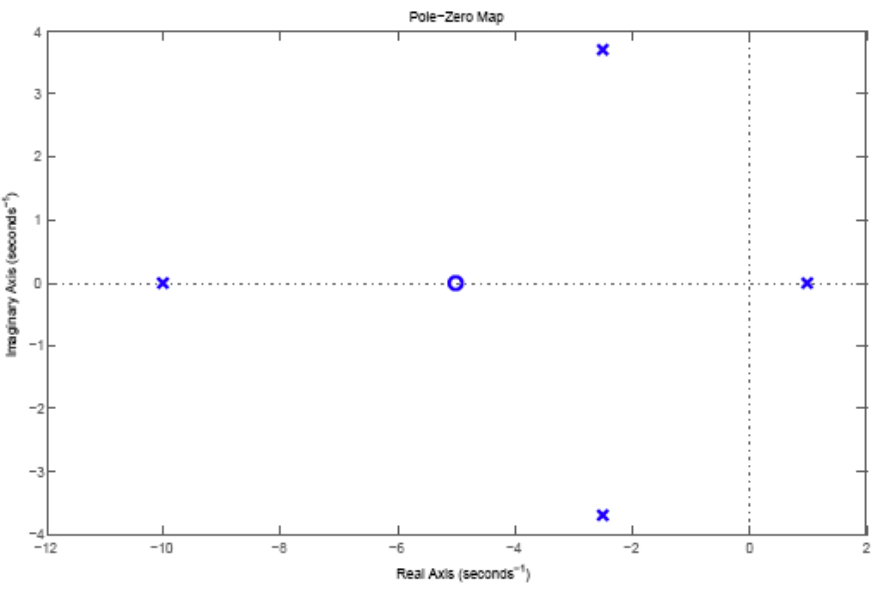
\includegraphics[scale=0.4]{immagini/polezero}
	\caption{Pole-zero map of G(s)}
	\label{fig:polezero}
\end{figure}
In the controllable canonical form the system can be decomposed in the following matrices:
\begin{equation*}
	A=\begin{bmatrix}
		0 & 1 & 0 & 0 \\
		0 & 0 & 1 &  0 \\
		0 & 0 & 0& 1 \\
		200& -130 & -55 & -14 \\
	\end{bmatrix}\quad 
	B=\begin{bmatrix}
		0	\\
		0	\\
		0\\
		1
	\end{bmatrix}
\end{equation*}
\[C=-\begin{bmatrix}
2000&400  & 0 & 0 
\end{bmatrix}
\]
Recall that the $\beta$ coefficients of the switching function [n=4]
\[s(x):=\beta_{n-1}x_1+\beta_{n-2}x_2+\dots+\beta_1x_{n-1}+x_n-\bar{w}\]
appear in the characteristic polynomial of the linear system S* of order 3 governing the dynamics of S when restricted to the sliding surface $s(x) = 0$:\[\chi^*(\lambda)=\lambda^{n-1}+\beta_1\lambda^{n-2}+\dots+\beta_{n-1}\]If we set the eigenvalues of S* equal to those stable of S
\[
\chi^*(\lambda)=(\lambda^2+5\lambda+20)(\lambda+10)=\lambda^3+15\lambda^2+70\lambda+200
\] then \[
 \beta'=\begin{bmatrix}
	\beta_3 & \beta_2 & \beta_1 & 1
	\end{bmatrix}=\begin{bmatrix}
200 &70 & 151 & 1
	\end{bmatrix}\] So that $\gamma=\frac{\beta_3}{b_4}=-0.1$ and $\alpha':= \beta'A=\begin{bmatrix}
	200 & 70 & 15 & 1
\end{bmatrix}$
Referring the following scheme the dynamics of some variables are plotted.
\begin{figure}[H]
	\centering
	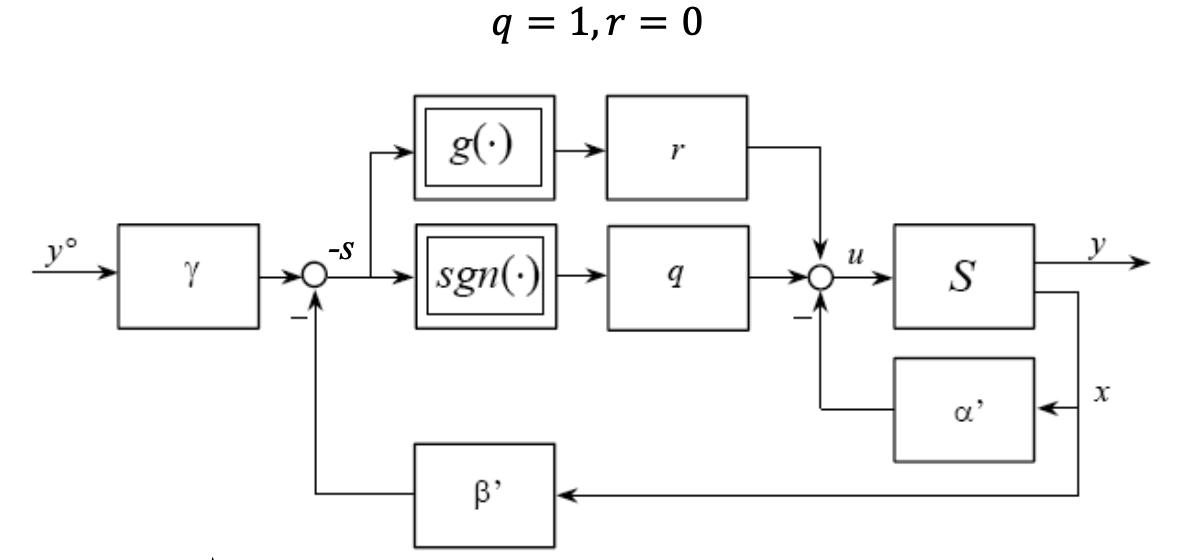
\includegraphics[scale=0.4]{immagini/ner}
	\caption{}
	\label{fig:ner}
\end{figure}
\begin{figure}[H]
	\centering
	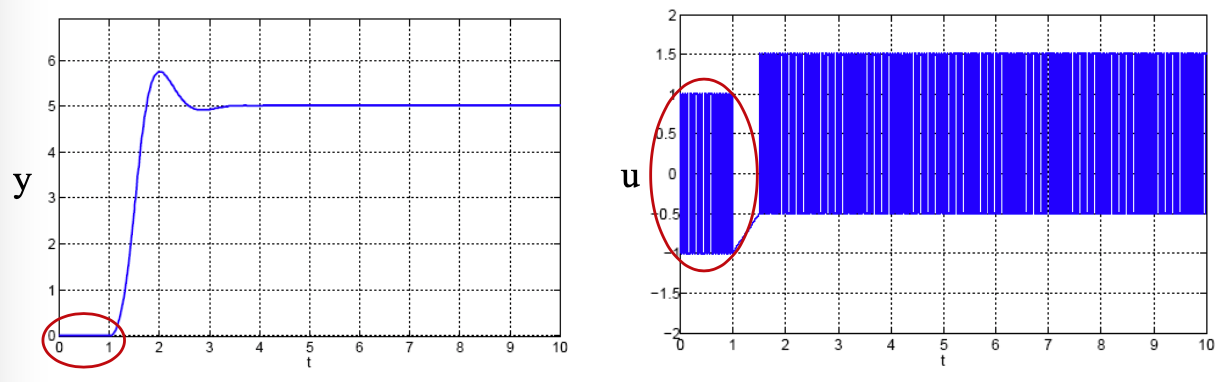
\includegraphics[scale=0.4]{immagini/ne1}
	\caption{$y°=5step(t-1), q=1[B_{MB/2}=0.02,M_{MB/2}=1]$}
	\label{fig:ne1}
\end{figure}
The system is initially on the sliding surface corresponding to y°=0, at the quasi-equilibrium with $\bar{y}=y°=0$, and keeps sliding on in the time interval [0,1).When $y°=5$, we have a different sliding surface. The time needed for reaching it satisfies $t_r\le\frac{|s(x(1))|}{q}$
\begin{figure}[H]
	\centering
	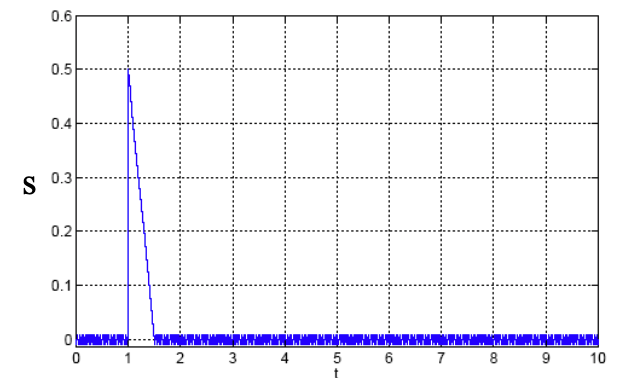
\includegraphics[scale=0.4]{immagini/ne2}
	\caption{$t:_r\le\frac{|s(x(1))|}{q}=0.5$}
	\label{fig:ne2}
\end{figure}
Changing the hysteresis threshold form 0.02 to 0.1 we obviously see a slower switching but same duration of reaching phase.

\begin{figure}[H]
	\centering
	\begin{subfigure}[b]{0.3\textwidth}
		\centering
		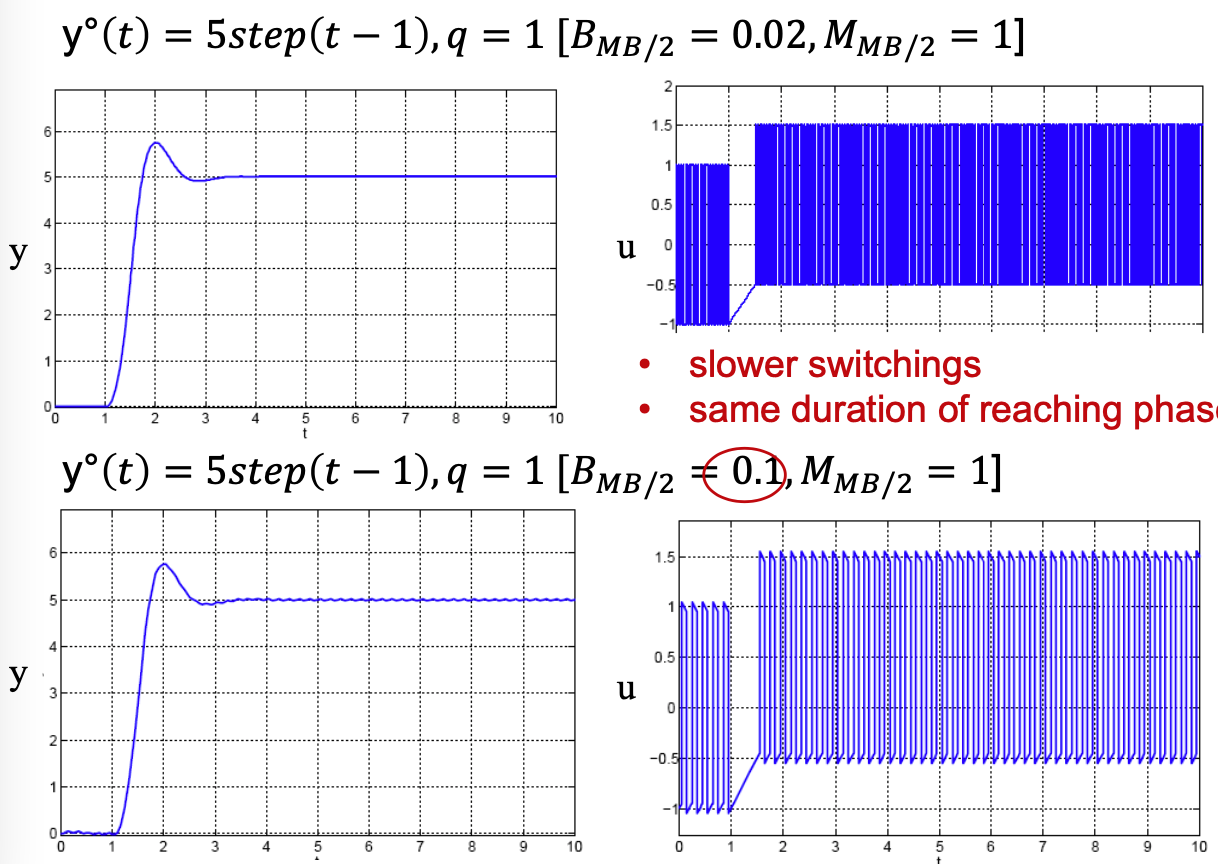
\includegraphics[scale=0.25]{immagini/ne3}
		\caption{y and u response}
		\label{fig:ne3}
	\end{subfigure}
	\hfill
	\begin{subfigure}[b]{0.3\textwidth}
		\centering
		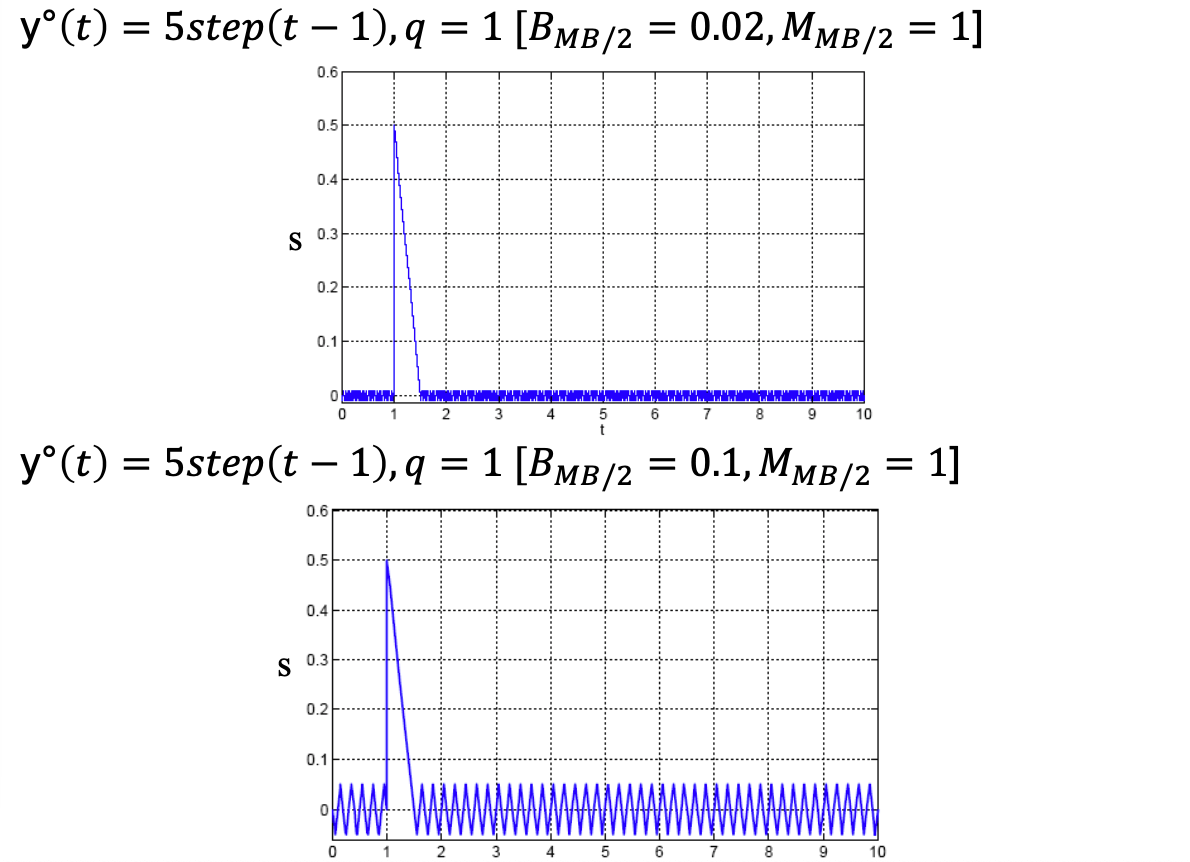
\includegraphics[scale=0.25]{immagini/ne4}
		\caption{s response}
		\label{fig:ne4}
	\end{subfigure}
	\hfill
	\label{fig:ne34}
	\caption{behaviour at different switching rate}
\end{figure}
We increase the step size for visual reason:
\begin{figure}[H]
	\centering
	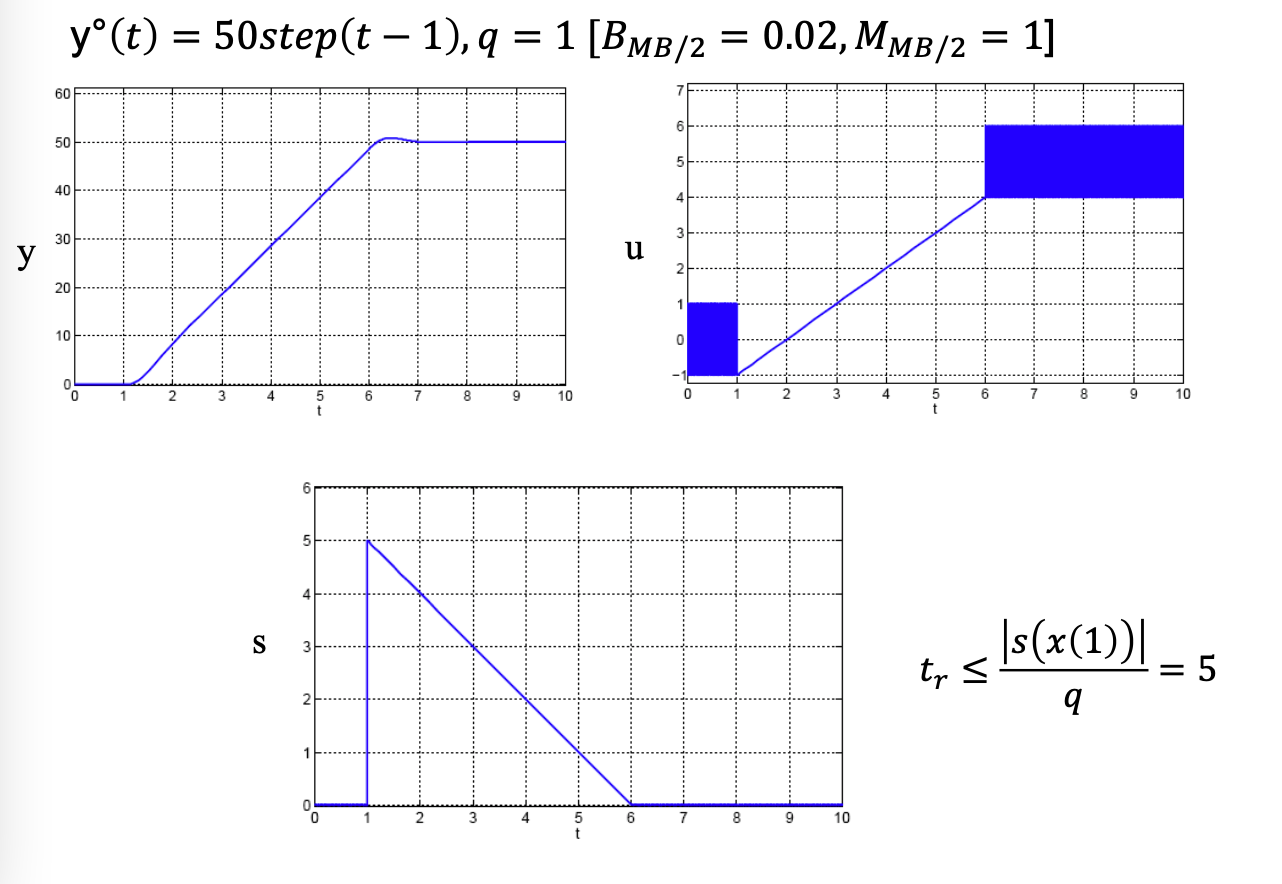
\includegraphics[scale=0.4]{immagini/ne5}
	\caption{Step size augmented to 50}
	\label{fig:ne5}
\end{figure}

While operating on the parameter \emph{''q''}, increasing it we notice a smaller duration of the reaching phase but a larger amplitude of u excursion (from 6 to 8 in this example).
\begin{figure}[H]
	\centering
	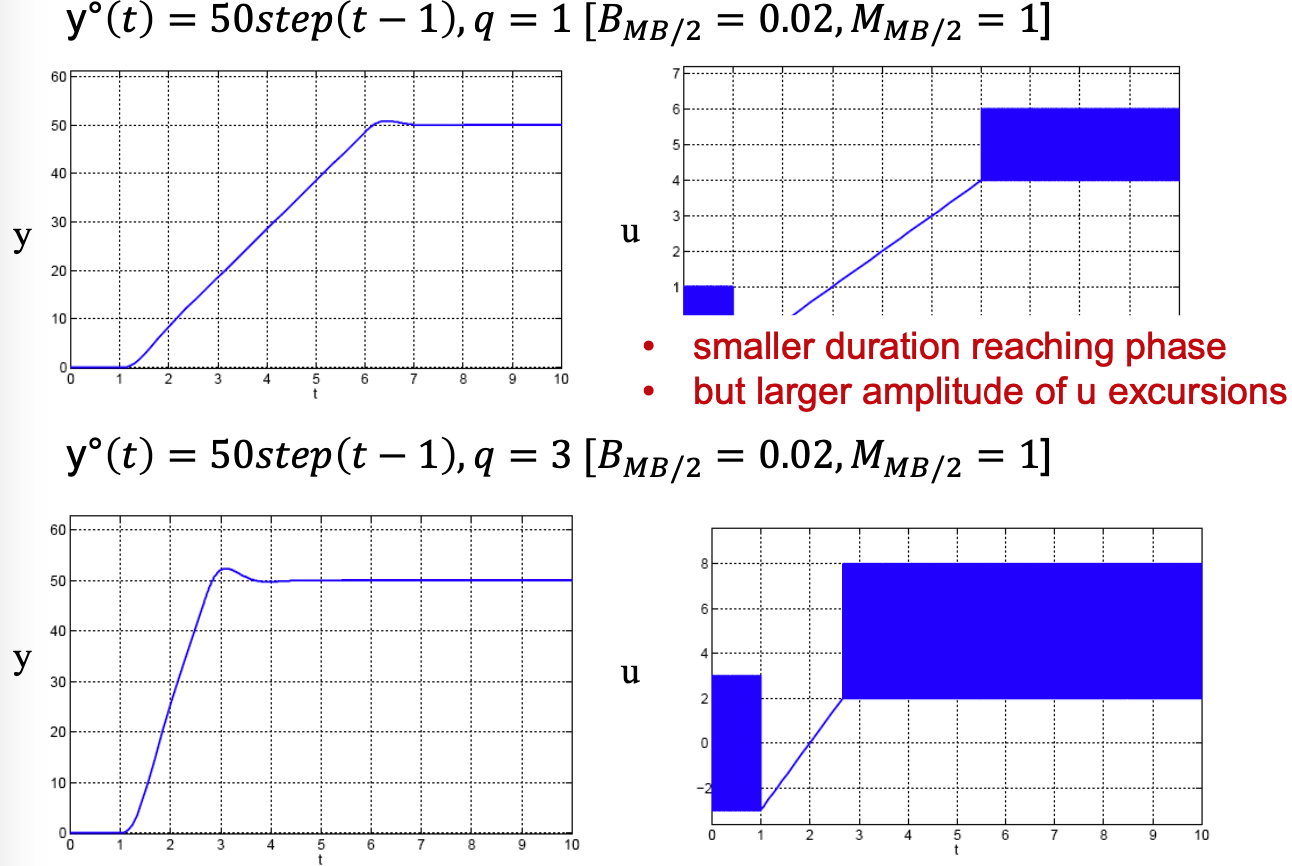
\includegraphics[scale=0.4]{immagini/ne6}
	\caption{}
	\label{fig:ne6}
\end{figure}
The question now is: how can one reduce the duration of the reaching phase, while do not affecting the u excursion? \\One can use an appropriate $g(\cdot)$ function. Take, e.g., $g(s)=s,\qquad \forall s\in \Re; \qquad r=1$.
\begin{figure}[H]
	\centering
	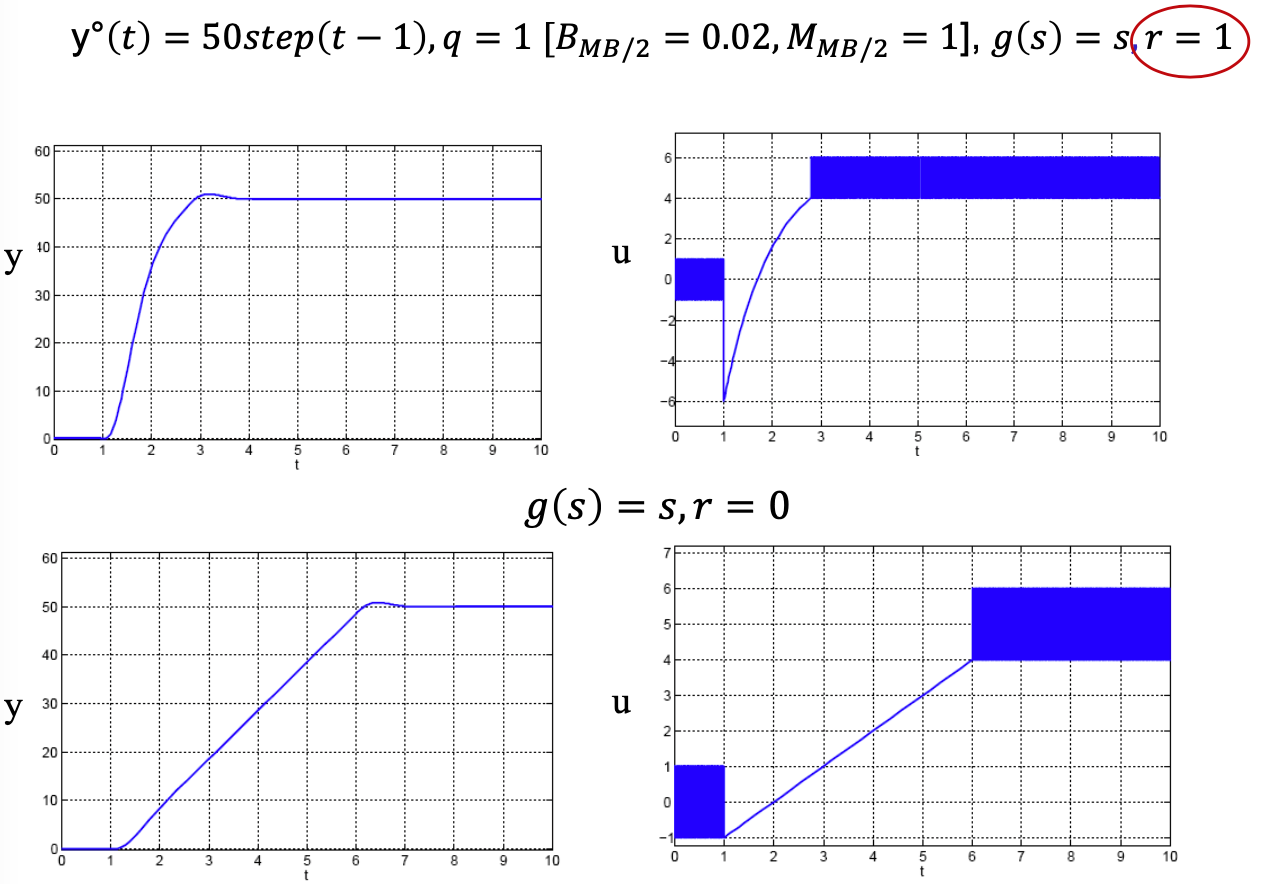
\includegraphics[scale=0.4]{immagini/ne7}
	\caption{}
	\label{fig:ne7}
\end{figure}
\section{State not available}
If the state is not directly measurable, given the transfer function G(s):
\begin{itemize}
	\item Refer to the minimal state space realization in controllable form for designing the variable structure control law as if the state were available \[u=-\alpha'x+q\,sgn(\gamma y°-\beta'x)+r\,g(\gamma y°-\beta' x)\]
	\item Introduce an asymptotic state observer (Luenberger observer) and use $\hat{x}$ in place of x in the sliding mode control law: \[
	u=-\alpha'\hat{x}+q\,sgn(\gamma y°-\beta'\hat{x})+r\,g(\gamma y°-\beta' \hat{x})
	\]
\end{itemize}
\begin{figure}[H]
	\centering
	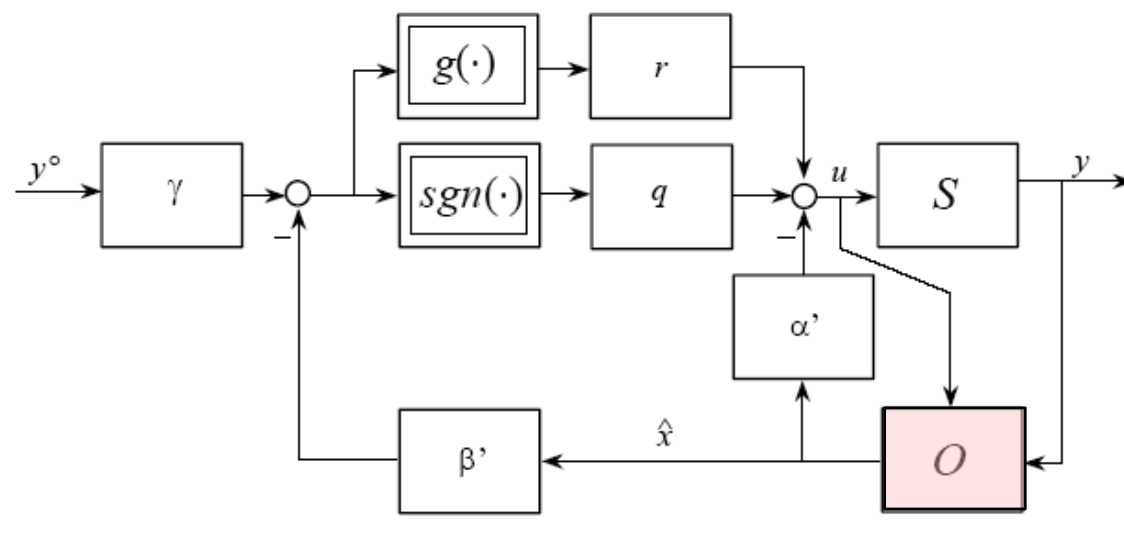
\includegraphics[scale=0.4]{immagini/nero}
	\label{fig:nero}
\end{figure}
\subsection{Numerical example}
Referring to the previous example, recalling the system transfer function 
\[
G(s)=\frac{-400(s+5)}{(s^2+5s+20)(s+10)(s-1)}=\frac{-400(s+5)}{s^4+14s^3+55s^2+130s-200}
\]Since the state is not directly measurable, we resort to the asymptotic observer (Luenberger observer) and use $\hat{x}$ in place of x in the sliding mode control law:
\[
u=-\alpha'\hat{x}+q\,sgn(\gamma y°-\beta'\hat{x})+rg(\gamma y°-\beta' \hat{x})
\]
Recalling the structure and the definition of observer
\begin{figure}[H]
	\centering
	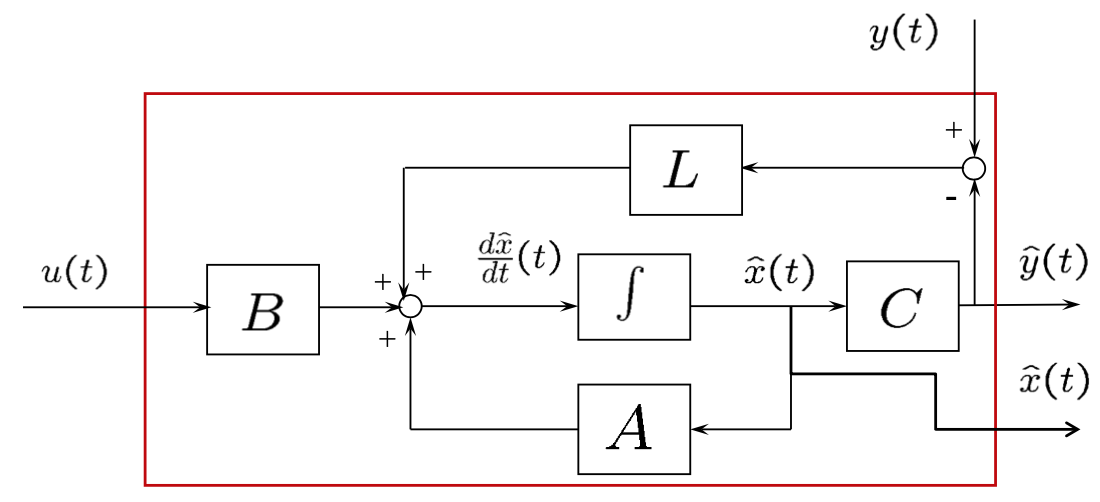
\includegraphics[scale=0.4]{immagini/observer6}
	\caption{$\dot{e}(t)=(A-LC)e(t)$}
	\label{fig:observer6}
\end{figure}
If (A,C) is observable, then, L can be designed so that A-LC has arbitrarily chosen eigenvalues and
the estimation error converges exponentially to zero with rate $\lambda_0\in(0,min|\Re{\lambda_i(A-LC)}|)$
\[\|e(t)\|\le\mu e^{-\lambda_0t}\|e(0)\|,t\ge0,\qquad \forall e(0)=e_0\in \Re^n\]
\begin{figure}[H]
	\centering
	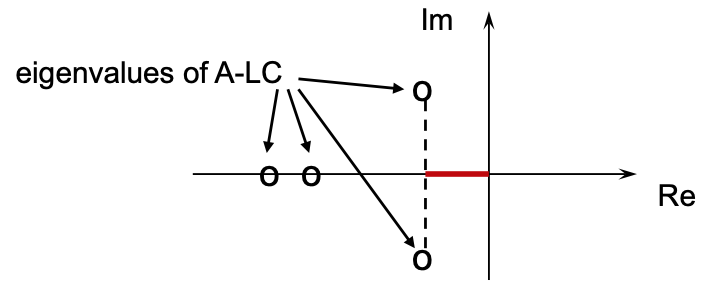
\includegraphics[scale=0.4]{immagini/eigenob}
	\label{fig:eigenob}
\end{figure}
If we choose the eigenvalues -10, -8, -6, -5 for the observer dynamics, we get: \[
L=\begin{bmatrix}
	-0.0025 & -0.0250 & 0.0175 & 0.2550
\end{bmatrix}'
\] and $0<\lambda_0<5$. 
\begin{figure}[H]
	\centering
	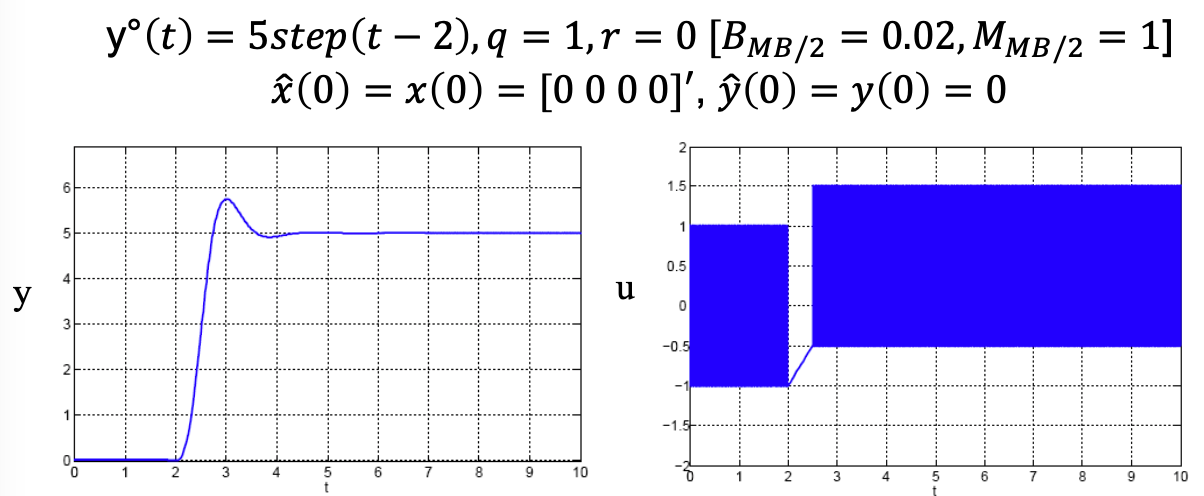
\includegraphics[scale=0.4]{immagini/ne8}
	\caption{}
	\label{fig:ne8}
\end{figure}
Same behaviour as without the observer since the estimation error is zero at time 0 and then keeps being zero.
\begin{figure}[H]
	\centering
	\begin{subfigure}[b]{0.3\textwidth}
		\centering
		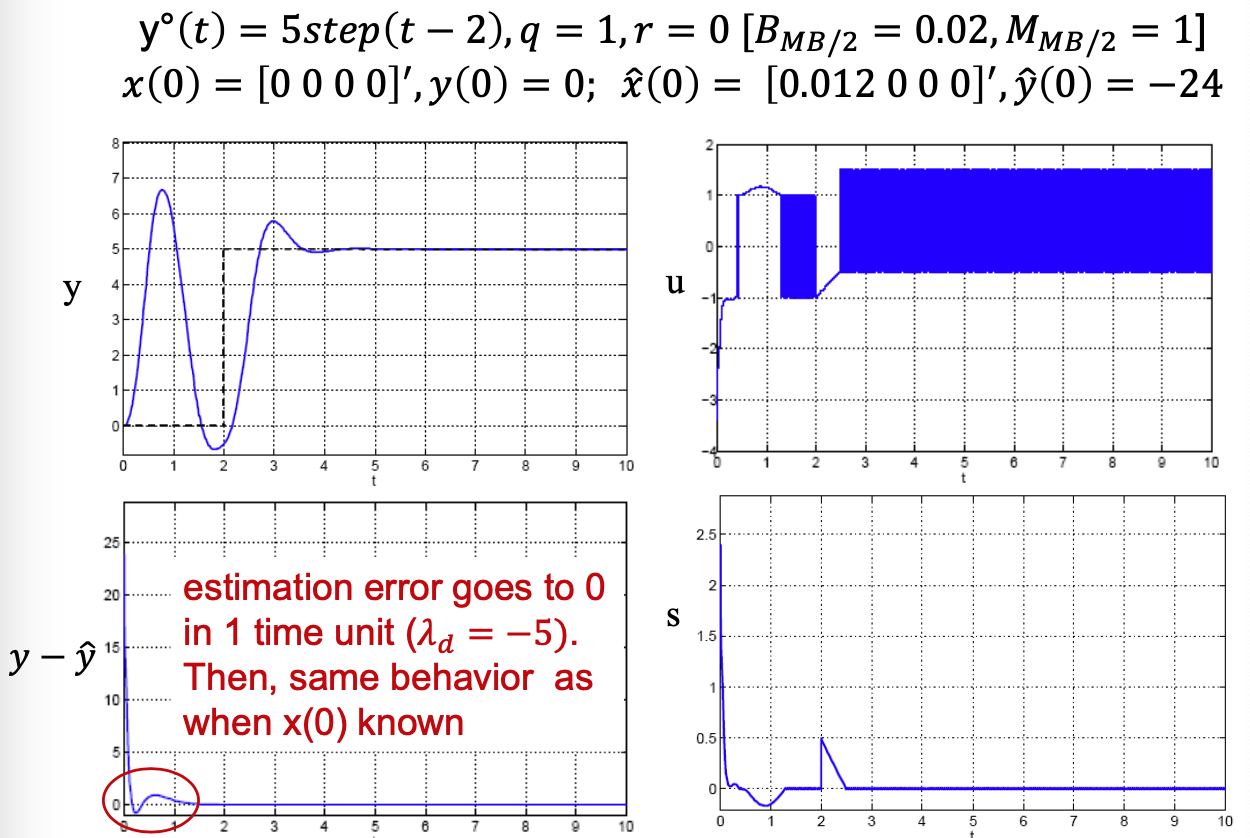
\includegraphics[scale=0.25]{immagini/ne9}
		\label{fig:ne9}
	\end{subfigure}
\hfill
	\begin{subfigure}[b]{0.3\textwidth}
		\centering
		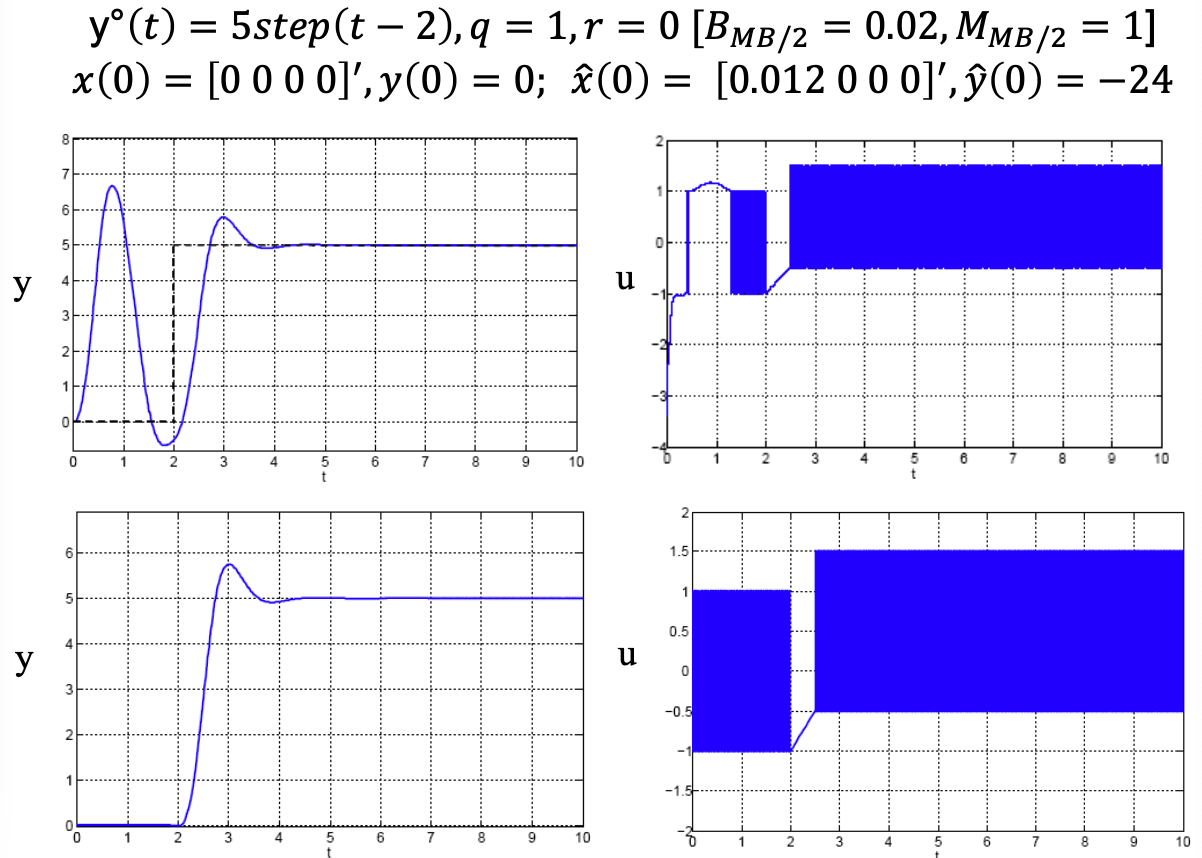
\includegraphics[scale=0.25]{immagini/ne10}
		\label{fig:ne10}
	\end{subfigure}
\hfill
\end{figure}
We have seen that in order to decrease the transient time $t_r$ and so making the switching faster we may increase $q$. But an higher $q$ means higher oscillation which are not desired. Let's analyze better this problem.
\section{Issue of the high frequency input switching}
The high frequency switching of the control input in the sliding mode phase can be undesirable and even unacceptable.
Possible solution:\\
filtering the high frequency components of the control input by introducing an \textcolor{red}{auxiliary control variable \emph{v} whose integral is the actual control variable \emph{u}}. In practice an integrator is added which has the aim to filter the control variable $u$.
\begin{figure}[H]
	\centering
	\includegraphics[scale=0.6]{"immagini/high freq"}
	\label{fig:high-freq}
	\caption{}
\end{figure}
Since now our plant is augmented we have $S$ in series with $\frac{1}{s}$ and since S is controllable canonical form we have to manage to put also $S^+$ in controllable canonical form through an appropriate transformation. And then we express our variable structure control law as a function of the original x variable by applying the reverse mapping.
\paragraph{Numerical example-continuous}
Let's write the transfer function of $S^+$, which is still controllable and observable system with no pole-zero cancellations: \[
G(s)=\frac{-400s-2000}{s^5+14s^4+55s^3+130s^2-200s}=\frac{10(1+0.2s)}{s(1+0.25s+0.05s^2)(1-s)(1+0.1s)}
\]
The enlarged controlled system can be written as
\[
S^+:\begin{cases}
	\dot{u}=v\\
	S:\begin{cases}
		\dot{x}=Ax+Bu\\
		y=Cx
	\end{cases}
\end{cases}
\]
and calling $z:=\begin{bmatrix}
	x' & u
\end{bmatrix}$' we have:
\[
S^+:\begin{cases}
	\dot{z}=Fz+Gv\\
	y=Hz
\end{cases}
\]
with \[
F:=\begin{bmatrix}
	A & B \\ 0 & 0
\end{bmatrix}, \qquad G:=\begin{bmatrix}
0 \\ 1
\end{bmatrix},\qquad H=\begin{bmatrix}
C & 0
\end{bmatrix}
\] which are not in controllable form. We can also notice that B became a state variable. Let's recover the controllable canonical form through some transformation matrices.
\[
	T=\begin{bmatrix}
		1 & 0 & 0 & 0 & 0 \\
		0 & 1 & 0 & 0 & 0 \\
		0 & 0 & 1 & 0 & 0 \\
		0 & 0 & 0 & 1 & 0 \\
		200 & -130 & -55 & -14 & 1
	\end{bmatrix},\qquad [T=\tilde{M}_CM_C^{-1}]
\]
\[
	\tilde{F}=TFT^{-1}\begin{bmatrix}
	0 & 1 & 0 & 0 & 0 \\
	0 & 0 & 1 & 0 & 0 \\
	0 & 0 & 0 & 1 & 0 \\
	0 & 0 & 0 & 0 & 1 \\
	0 &200 & -130 & -55 & -14 
\end{bmatrix},\qquad  \tilde{G}=TG=G
\]
\[\tilde{H}=HT^{-1}=\begin{bmatrix}
	-2000 & -400 & 0 & 0 & 0
\end{bmatrix}\]

Dynamics within the sliding surface:
\[\chi^*(\lambda)=(\lambda^2+5\lambda+20)(\lambda+10)^2=\lambda^4+25\lambda^3+220\lambda^2+900\lambda+2000\]
\[
\begin{aligned}
		&\tilde{\beta}^{+'}:=\begin{bmatrix}
			\tilde{\beta}^+_4 & \tilde{\beta}^+_3 & \tilde{\beta}^+_2 & \tilde{\beta}^+_1 & 1
		\end{bmatrix}\\
	&\tilde{\alpha}^{+'}:=\tilde{\beta}'\tilde{F}=\begin{bmatrix}
		0 & 2200  &770 & 165 & 11
	\end{bmatrix}\\
	&\tilde{\beta}^+_5=\tilde{H}(1,1)=-2000,\qquad \gamma^+=\frac{\tilde{\beta}^+_4}{\tilde{b}^+_5}=-1
\end{aligned}
\]while going back to the original state variables were:
\[
\begin{aligned}
	&\beta^{+'}=\tilde{\beta}^+T=\begin{bmatrix}
		2200 & 770 & 165 & 11 & 1
	\end{bmatrix}\\
&\alpha^{+'}=\tilde{\alpha}^+T=\begin{bmatrix}
	2200 & 770 & 165 & 11 & 11
\end{bmatrix}
\end{aligned}
\]Once we have all the coefficients this is what happens. To remind us, v is the input to $S^+$ system referencing to Figure 6.20. The integration system is initialized with 0 in the beginning and we see that when we take the integral of v, which is oscillating, we get a smoother line. If at the beginning we have the mean (which is 0) after the switching signal we get a constant because in the meantime something has been integrated. So the actual input to our system is not anymore the one we get directly the variable structure controller  to the system but it is a filtered version which is smooth.
\begin{figure}[H]
	\centering
	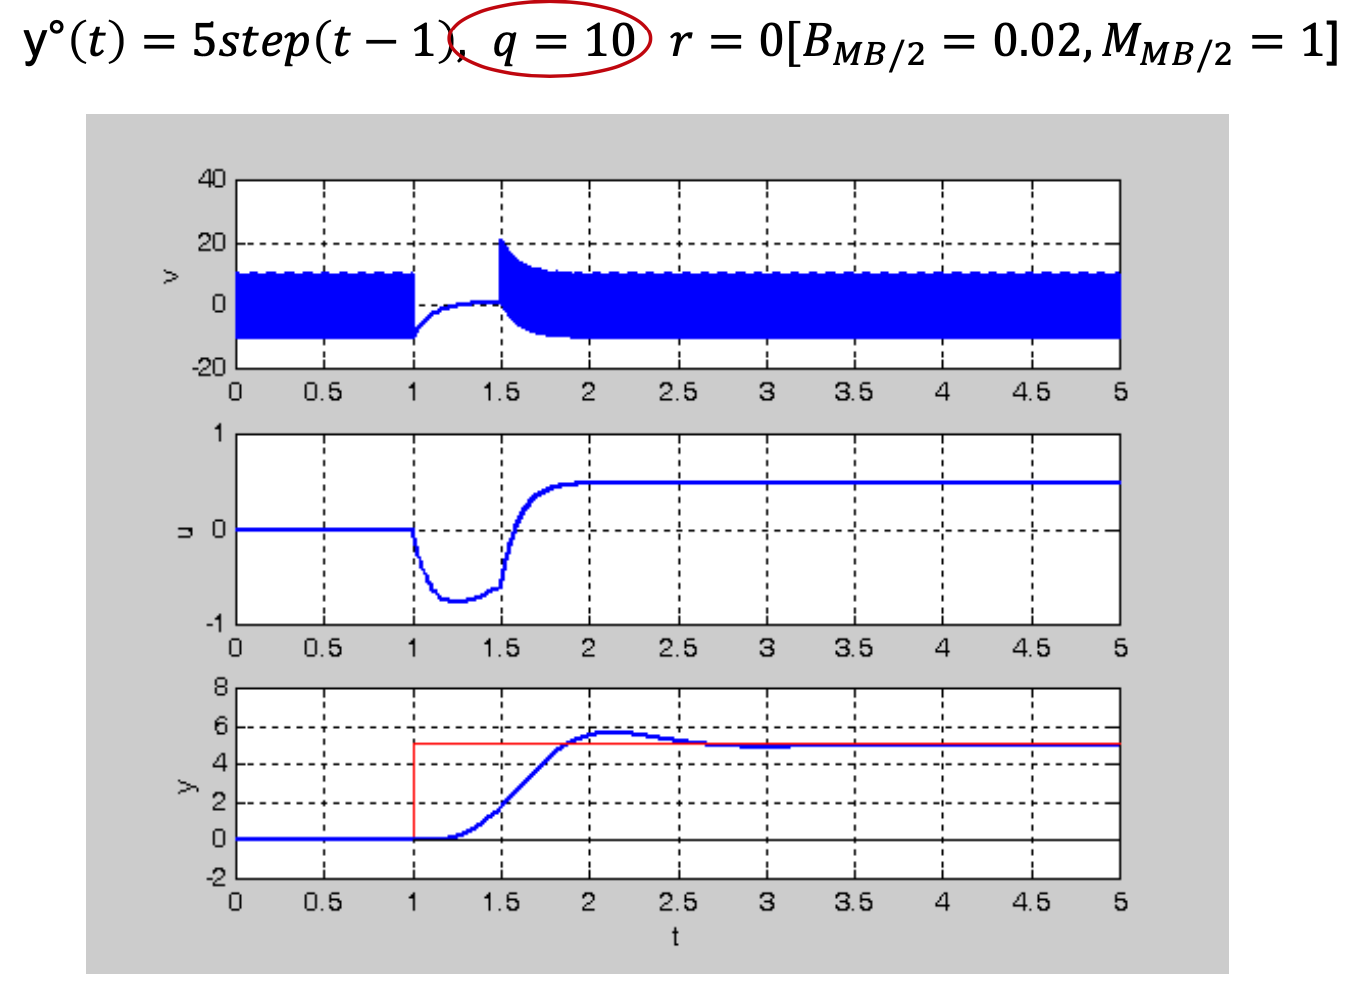
\includegraphics[scale=0.4]{immagini/vscnumex}
	\caption{}
	\label{fig:vscnumex}
\end{figure}
\section{Robustness with respect to parameter uncertainty}
We shall now evaluate:
\begin{itemize}
	\item robustness of the control strategy with respect to parameter uncertainty
\end{itemize}
We shall fix $r=0$, for simplicity. We will consider the following system: \[
G_1(s)=\frac{-150(s+10)}{s^4+14s^3+55s^2+30s-100}
\]associated to the following pole zero map. 
\begin{figure}[H]
	\centering
	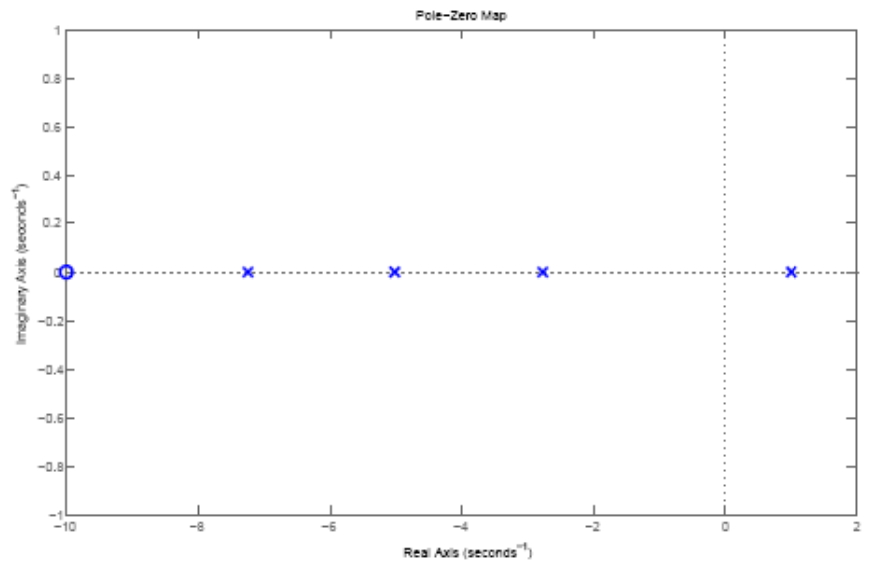
\includegraphics[scale=0.4]{immagini/polezeromap}
	\caption{Pole-Zero map}
	\label{fig:polezeromap}
\end{figure}
Let's see what happens applying the variable structure control designed for the previous system  \[
G(s)=\frac{-400s-2000}{s^5+14s^4+55s^3+130s^2-200s}=\frac{10(1+0.2s)}{s(1+0.25s+0.05s^2)(1-s)(1+0.1s)}
\] which is different. What happens is actually that we don't reach anymore the correct equilibrium but a wrong one because the coefficient $b_n$ changed from -200 to a -100 and $\gamma$ depends on it.
\begin{figure}[H]
	\centering
	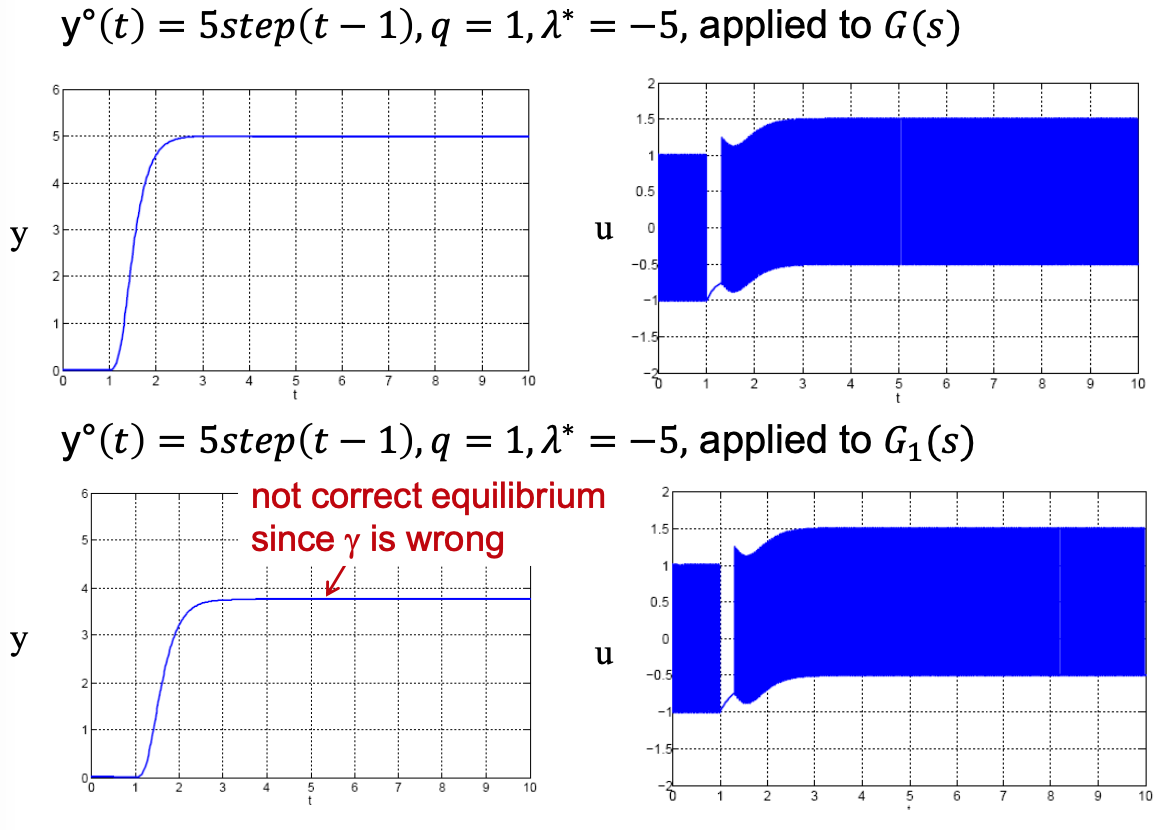
\includegraphics[scale=0.4]{immagini/g1gconf}
	\caption{}
	\label{fig:g1gconf}
\end{figure}



\begin{figure}[H]
	\centering
	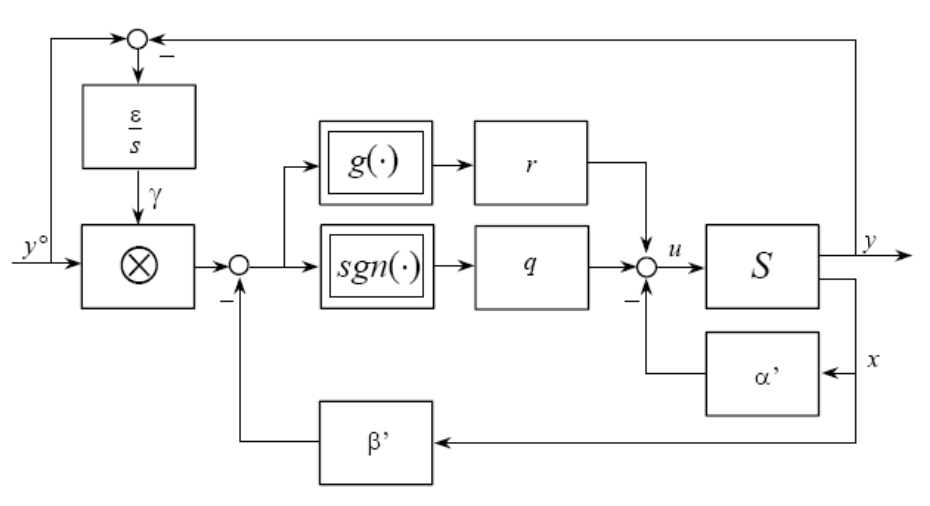
\includegraphics[scale=0.4]{immagini/adaptgamma}
	\caption{Scheme with the adaptation of the gain $\gamma$}
	\label{fig:adaptgamma}
\end{figure}
\section{Robustness with respect to load disturbance}
Suppose now, that S is subjected to some load disturbance $w(t)$.
\begin{figure}[H]
	\centering
	\includegraphics[scale=0.4]{immagini/robloaddist}
	\caption{Load disturbance $w(t)$}
	\label{fig:robloaddist}
\end{figure}
The intuition here why this scheme is robust against load disturbances is: the $\dot{s}$ function is pushing \emph{s} towards 0 with the strength that keeps within \emph{q} even if \emph{s} goes to zero. So if this disturbance is attenuating the contribution of \emph{q} but never exceeding the value of \emph{q} we are  still pushing \emph{s} to become zero and get the desired behaviour. Let's prove it formally.\\
\underline{Statement:}\\
If $|w(t)|\le W<q, \forall t$, then the state will reach sliding surface $s(x)=\tilde{y}-\gamma y°=0$ in finite time and will evolve according to the desired dynamics of $S^*$. \\\underline{Only the time to converge is affected by \emph{w}}.
\begin{proof}
	Consider $V(s)=\frac{1}{2}s^2$, where $s=\tilde{y}-\gamma y°$.\\ Then, \[\frac{dV}{dt}=s\dot{s}=s\dot{\tilde{y}}\] Since $\dot{\tilde{y}}=v+w$ (to be shown after) and $v=-q\, sgn(s)-r\,g\,(s)$.\\ Then \[\frac{dV}{dt}=s\dot{s}=s\dot{\tilde{y}}=-s\,q\,sgn(s)-s\,r\,g(s)+sw\]
	since $s\,g(s)>0$ can be neglected for the upperbounding and $|w|\le W(<q)$ implies that $sw \le W|s|$ we get the upper bound \[\frac{dV}{dt}=-s\,q\,sgn(s)-s\,r\,g(s)+sw\le -(q-W)|s|.\] This implies that, for any initial condition $x(0),s(x(t))$ converges to zero in a finite time $t_r\le \frac{|s(x(0))|}{q-W}$.\\When the sliding surface  $s(x)=\beta'x-\gamma y°=\tilde{y}-\gamma y°=0$ is reached , then, the system evolves on the sliding surface according to the dynamics of $S^*$ so the output \emph{y} tends to \emph{y°}. At this point we just need to show that \[\dot{\tilde{y}}=v+w\] (we gave for granted before).\\
We exploit the sub-system $\bar{S}$ as follow and derive the state space equation and then compute the transfer function.
\[\bar{S}:\begin{cases}
	\dot{x}=Ax+Bu\\
	\tilde{y}=\beta'x
\end{cases},\qquad u=v+w-\alpha'x
\] \[\Downarrow\]
\[\bar{S}:\begin{cases}
	\dot{x}=Ax+B(v+w)\\
	\tilde{y}=\beta'x
\end{cases}\qquad \tilde{A}=A-B\alpha'
\] where

$\beta':=\begin{bmatrix}
	\beta_{n-1} & \beta_{n-2} & \dots & \beta_1 & 1
\end{bmatrix}
$,
\[
A:=\begin{bmatrix}
	0 & 1 & 0 & \dots & 0 \\
	0 & 0 & 1 &  \dots & 0 \\
	0 & 0 & 0 & 0 & 0 \\
	\vdots& \vdots & \vdots & \vdots & \vdots \\
	0& 0 & 0 & 0 & 1 \\
	-\alpha_n &-\alpha_{n-1} & -\alpha_{n-2} & \dots & -\alpha_1 
	\end{bmatrix}B= \qquad\begin{bmatrix}
	0 \\
	0 \\
	0 \\
	\vdots \\
	0 \\
	1
\end{bmatrix}
\]\[\Downarrow\]\[\alpha':=\beta'A=\begin{bmatrix}
	-a_n & \beta_{n-1}-a_{n-1} & \beta_{n-2}-a_{n-2} & \dots & \beta_1 -a_1
\end{bmatrix}
\]and so
\[
\tilde{A}=\begin{bmatrix}
	0 & 1 & 0 & \dots & 0 \\
	0 & 0 & 1 &  \dots & 0 \\
	0 & 0 & 0 & 0 & 0 \\
	\vdots& \vdots & \vdots & \vdots & \vdots \\
	0& 0 & 0 & 0 & 1 \\
	0 & -\beta_{n-1} & -\beta_{n-2} & \dots & -\beta_2 & -\beta_1
\end{bmatrix}
\]
\[
\tilde{G}(s)=\frac{s^{n-1}+\beta_1s^{n-2}+\dots+\beta_{n-1}}{s^n+\beta_1s^{n-1}+\beta_2s^{n-2}+\dots+\beta_{n-1}s}=\frac{\chi^*(s)}{s\chi^*(s)}=\frac{1}{s}
\]When we have a transfer function of a linear system if the number of the poles is  not equal to the order means that there is something hidden which is either  non controllable or non observable or both of them.	Since this is in the controllable canonical form the system must be controllable and the hidden part in consequence is in the non-observability subspace.
System $\bar{S}$:
\begin{itemize}
	\item[-] externally $v+w\to\textasciicaron{y}$ behaves like an integrator \[\dot{\tilde{y}}=v+w\]
	\item[-] has hidden a.s. dynamics with characteristic polynomial $\chi^*(s)$
\end{itemize}
\end{proof}

%%%% Fine del Capitolo %%%